






% =========----------	[ Space left here for distraction free mode] ----------==========%










\section{Recording at Abbey Road Studios}
	% - Description of recording process
	% - Band + song
	% - List of microphones arrays + positions

	The following section describes the planning process and recording session of this project. All microphones arrays used in the recording session are listed and described including their position within the room. 

	\subsection{Planning}
		% The Band - 5 piece indie rock band that can be spread out across the room
		To produce a VR experience of a live musical performance an appropriate musical ensemble was required. There were a few prerequisites before deciding upon an ensemble, such as deciding upon a musical genre. The style of music needed to be appropriate for a wider demographic and could not be explicit in its nature. The ensemble must also be well-rehearsed and employ a sense of professionalism to ensure that the time available in the studio was used efficiently and productively. With these conditions in place, a London-based Indie-Pop ensemble called 'Nova Neon' were contacted. Nova Neon are a five-piece band who play a sophisticated style of Indie-Pop using a mix of both anechoic sounds and acoustic instruments. The song chosen for the performance was called 'Close Your Eyes' from their album 'Chroma'. This song was chosen for the hard panned left and right guitars which could be exaggerated within an Higher-Order Ambisonic reproduction. \\

		% The room - Studio 3 is large enough to house the band and has heigh ceilings

		The recording location of choice was Studio Three at Abbey Road Studios. The room is large enough to comfortably house the 5 piece band and boasts heigh ceilings that allow for a more diffuse sound-field to exist higher in the room which could be taken advantage of in exploring capturing the ambience of the space using dedicated multichannel microphone arrays.\\


	\subsection{Microphone and Camera Set Up}

		As this research is currently of interest amongst audio engineers and professionals in the audio industry, it was decided to invite other collaborators to participate in the research. Dr Hyunkook Lee from Huddersfield University was invited to attend the recording session to set-up the Equal Segment Microphone Array, which he had shown to perform well at capturing audio for VR. The technical director of Schoeps Mikrofone Helmut Wittek was also contacted with an invitation to collaborate. Schoeps agreed to contribute by supplying their ORTF-3D Surround and OCT-9 Surround multichannel microphone arrays (MMAs). By collaborating with Schoeps Mikrofone and Dr Hyunkook Lee, the research was expanded to include a wider selection of multichannel microphone arrays for subjective analysis. 

		% Floor Plan
		The floor plan for studio three can be seen in Figure~\ref{FloorPlan} annotated with three letters, A (green), B (red) and C (blue) showing the different positions that the Ambisonic microphones, multichannel microphone arrays and 360\textdegree{} video cameras were placed. \\

		% Musician Placement


		 The following sections list the microphones that were placed in each of these positions.

		\begin{figure}
			\begin{center}
				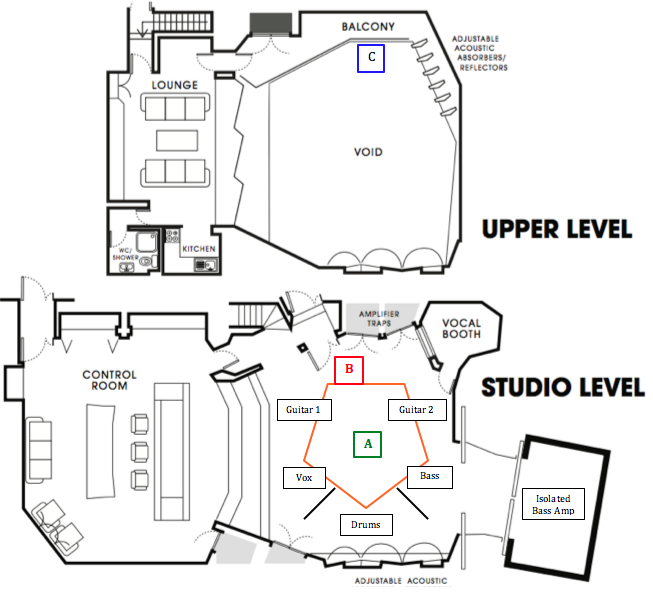
\includegraphics[width = 0.8\linewidth]{images/other/FloorPlan.png}
				\caption{Preliminary floor plan of the recording session in Studio Three \cite{Studio3}}
				\label{FloorPlan}
			\end{center}
		\end{figure}

		% List of all microphones + Cameras

		% Position A
		\subsubsection{Position A}

			Position A is located in the centre of recording space and in the middle of the musicians. This is where the visuals for the VR experience were captured in 360\textdegree{} using the GoPro Omnirig. The Soundfield ST450 MKII, EM32 Eigenmike, Equal-Segment-Microphone-Array (ESMA) and Schoeps ORTF3D Surround were also set-up in this position to capture direct sound radiating from the instruments.\\

			\paragraph{GoPro Omnirig}
			The GoPro Omnirig is a synchronised six-camera array used to capture 360\textdegree{} videos \cite{gopro}. It was placed at position A at a height of 160cm to the bottom of the array. GoPro number one in the Omnirig was positioned to face a reference point at the back wall where the drum kit would be set-up.\\

			\paragraph{Neumann KU100}
			The KU100 was positioned to be facing towards the reference point (drum kit). Though this would not be used in the listening tests  it was included so it could be used to compare against the other recording techniques.\\

			\paragraph{EM32 Eigenmike}
			The Eigenmike was placed on its side just above the GoPro Omnirig at a height of 1.81m shown in figure~\ref{STApos}. The aim was for the Eigenmike to capture the direct sound from the instruments and provide a soundfield recording 'canvas' on which the spot microphone recordings could be placed within a Higher-Order Ambisonic framework. \\

			\paragraph{Soundfield ST450 MKII}
			The soundfield microphone was placed at a height of 2m and placed on its side above the GoPro Omnirig and Eigenmike. It is worth noting that the 'end fire' switch must be activated on the ST450 pre-amplifier if the microphone is placed on its side for recording. The 'end fire' setting adjusts the X, Y and Z axis data to ensure that the correct soundfield orientation is captured.\\

			\begin{figure}[ht]
			\begin{center}
				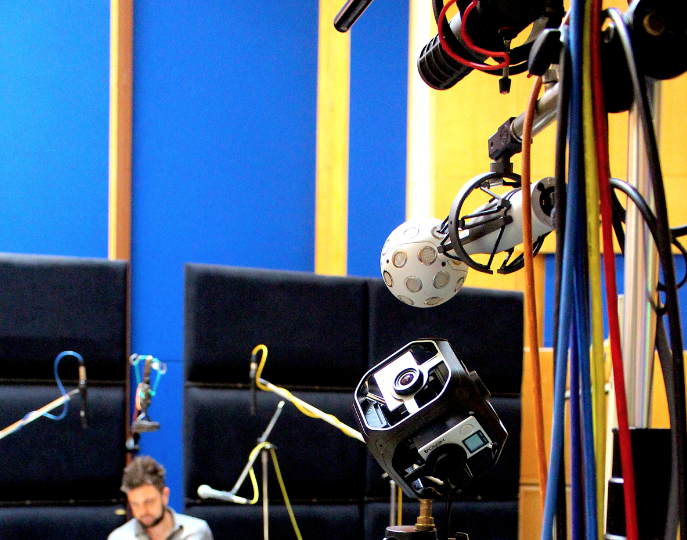
\includegraphics[width = \linewidth]{images/other/ST450pos.png}
				\caption{Placement of the first Soundfield ST450 MKII microphone, Eigenmike and GoPro Omnirig at position A}
				\label{STApos}
			\end{center}
			\end{figure}

			\paragraph{Equal Segment Microphone Array (ESMA)}
			The ESMA is based on the 'four segment array' proposed by Michael Williams in 1991 \cite{williamsMMAD}, \cite{williams91}. It was designed to capture sound from 360\textdegree{} in the azimuth plane using four cardioid microphones positioned in a square arrangement, with a distance of 25cm between each capsule. The angles between each microphone should be 90\textdegree, creating a stereophonic recording angle (SRA) of $ \pm45 $\textdegree \cite{williamsMMAD}, \cite{williams91}. 

			Through listening tests, Dr Hyunkook Lee of Huddersfield University found that by changing the distance between each capsule to 50cm, the localisation accuracy of sound sources within a VR environment was improved \cite{esma}. Each of the four microphones on the azimuth plane were angled down by 45\textdegree{} to face the instruments and optimise direct sound capture from the instruments. The array was positioned at a height of 2.15m, with the upward facing microphone capsules reaching a height of 2.28m. The four additional upward-facing cardioid microphones were added to capture some of the diffuse sound within the recording environment. The four upward-facing microphones were also set-up with distance of 50cm between each capsule. The use of cardioid microphones and the wide spacing between each microphone capsule helps to minimise inter-channel cross-talk, whilst still providing satisfactory localisation of sound sources within the azimuth plane.\\


			\paragraph{ORTF-3D Surround}
			The supercardioid microphones used in this array allow for sufficient signal separation between each microphone to avoid unwanted inter-channel cross-talk and comb-filtering effects. The spacing between each microphone follows the principles of the ORTF technique to allow for the required inter-channel time differences and improved spatial resolution to be included into the recording. The ESMA and ORTF can both be seen at position A in figure~\ref{esma}.\\


			\begin{figure}[h]
			\begin{center}
				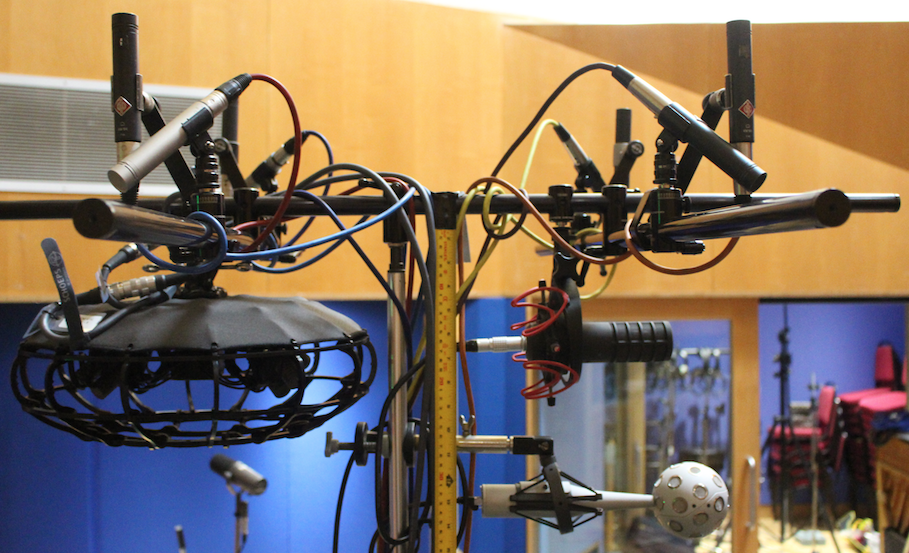
\includegraphics[width = \linewidth]{images/other/esmapic.PNG}
				\caption{Picture of the ORTF-3D Surround Array without windshield (top) and the ESMA (left) just underneath. The front of the arrays was positioned facing the reference point at the drum kit.}
				\label{esma}
			\end{center}
			\end{figure}

		% Position B
		\subsubsection{Position B}
			Position B is located to the rear of Studio Three near the entrance. The objective for this position was to capture a 180\textdegree{} view of the musicians and provide a different audio and visual perspective for the VR experience. The Samsung Gear 360 camera, Stereo X-Y pair, OCT-9 Surround, Perceptual Control Microphone Array (PCMA) and Sennheiser AMBEO Ambisonic microphone were placed at position B to capture both audio and video from this viewing (and listening) position.\\

			\paragraph{Samsung Gear 360}
			The Samsung 360 was used to provide a 180\textdegree{} visual perspective of the live performance with the musicians in front of the viewing position. The camera, multichannel microphone arrays and Ambisonic microphones were directed at the same reference point facing towards the drum kit. \\

			\paragraph{Stereo X-Y Pair}
			A coincident stereo X-Y microphone arrangement was set-up at position B as a reference. Two Neumann KM184 cardioid microphones were arranged to produce a stereo recording angle of 115\textdegree{} and positioned to face the drum kit at a height of 1.94m to the coincident point.\\

			\paragraph{Sennheiser AMBEO}
			The Sennheiser AMBEO is a B-format Ambisonic microphone similar to the Soundfield ST450 MKII. It is also capable of recording First-Order Ambisonics using a tetrahedral coincident arrangement of four cardioid microphone capsules \cite{ambeo}. The AMBEO is available to purchase at a considerably lower price compared to the Soundfield ST450 MKII and therefore it would be of interest to compare their performance. The AMBEO was placed at position B, just above the Samsung Gear 360 camera at a height of 1.59m to the centre of the microphone grill. The positioning of the AMBEO did cause some occlusion where the Samsung camera was obstructing sound from entering the bottom of the microphone, shown in figure~\ref{ambeopic}. This was not ideal but due to limited space available the positioning was deemed appropriate. \\
			
			\begin{figure}[h]
			\begin{center}
				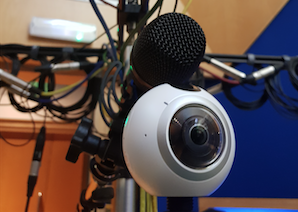
\includegraphics[width = \linewidth]{images/other/ambeopic.png}
				\caption{Placement of the Sennheiser AMBEO and Samsung Gear 360 camera at position B}
				\label{ambeopic}
			\end{center}
			\end{figure}

			\paragraph{Perspective Control Microphone Array (PCMA)}
			Due to space and equipment limitations encountered during the recording session, the PCMA set-up used the front-centre, rear-facing and upward-facing microphones from the OCT-9 Surround. Coincident stereo pairs were set-up for only the front left and front right positions. The PCMA was set-up at a height of 1.82m to the microphone capsules.\\

			\paragraph{OCT-9 Surround}
			The OCT-9 Surround microphone array was designed by G\"{u}nther Theile and Helmut Wittek for the Auro-3D (9.1) loudspeaker arrangement. The front facing section is based on Theile's optimised cardioid triangle surround (OCT-Surround) array, which is used to capture sound for 5.1 multichannel systems \cite{TheileWittek}, \cite{Theile}. Four upward-facing supercardioid microphones are added to the OCT-surround to create the complete OCT-9 Surround array. Using directional microphones in this way again helps to increase channel separation and avoid unwanted inter-channel cross-talk. The front three microphones are used to capture direct sound whilst the rear and upward-facing microphones capture the diffuse sound and ambience of the recording environment. \\



		% Position C
		\subsubsection{Position C}
			Position C was located behind position A at the rear of Studio Three. At position C, the IRT Cross, Hamasaki Cube and second Soundfield ST450 MKII microphone were placed much higher in the room in contrast to the multichannel microphone arrays located at positions B and C. The aim was for the height arrays and Ambisonic microphone in position C to record more of the diffuse sound existing higher up in the room and capture the ambience of the recording space.\\

			\paragraph{IRT Cross}
			The IRT cross or 'atmo-cross' is a multichannel microphone array generally used to capture diffuse sound and direct environmental sounds such as applause and crowd noise. It can be created using four cardioid microphones positioned in a square with 20cm - 25cm spacing between each capsule \cite{IRTschoeps}. The IRT Cross can also be used in combination with other arrays to allow for the capture of both direct and diffuse sound to provide a full spatial representation of a musical performance within an environment. The IRT Cross was positioned at a height of 3.5m at position C, which helped to reduce direct sound capture and increase the diffuse sound captured.\\


			\paragraph{Hamasaki Cube}
			The Hamasaki Cube is a multichannel microphone array specifically designed to capture the reverberation and diffuse sound in performance spaces such as concert halls. Due to space limitations, the dimensions of the Hamasaki Cube were reduced from 1m to 0.7m. Eight Neumann U87 condenser microphones were used to create the Hamasaki Cube, which was positioned at a height of 3m to the microphone capsules on the lower layer of the cube. The microphone capsules on the upper layer of the Hamasaki Cube reached a total height of 3.7m. Given the widely spaced microphone arrangement and the height of the Hamsaki Cube creating sufficient inter-channel time and level differences, it was expected to perform well at capturing the ambience Studio Three.\\

			\paragraph{Soundfield ST450 MKII}

			The second Soundfield ST450 MKII Ambisonic microphone was positioned between the front two microphones of the IRT Cross at a height of 3.45m to centre of the microphone grill. This allowed for a First-Order Ambisonic soundfield recording higher up in the recording space in the hope of capturing more of the rooms ambience. \\

			All three microphones at position C is illustrated in figure~\ref{pos3} and the separation between position A and C is shown in figure~\ref{AvsC}.\\

			\begin{figure}[h]
			\begin{center}
				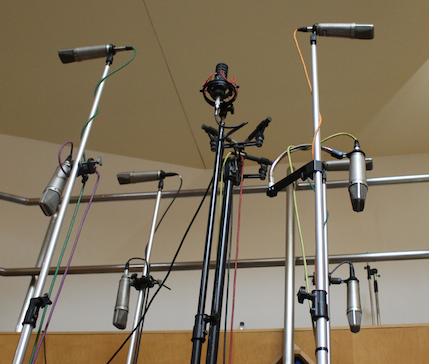
\includegraphics[width = \linewidth]{images/other/positionC.png}
				\caption{Placement of the second Soundfield ST450 MKII, IRT Cross and Hamasaki Cube at position C}
				\label{pos3}
			\end{center}
			\end{figure}

			\begin{figure}[h]
			\begin{center}
				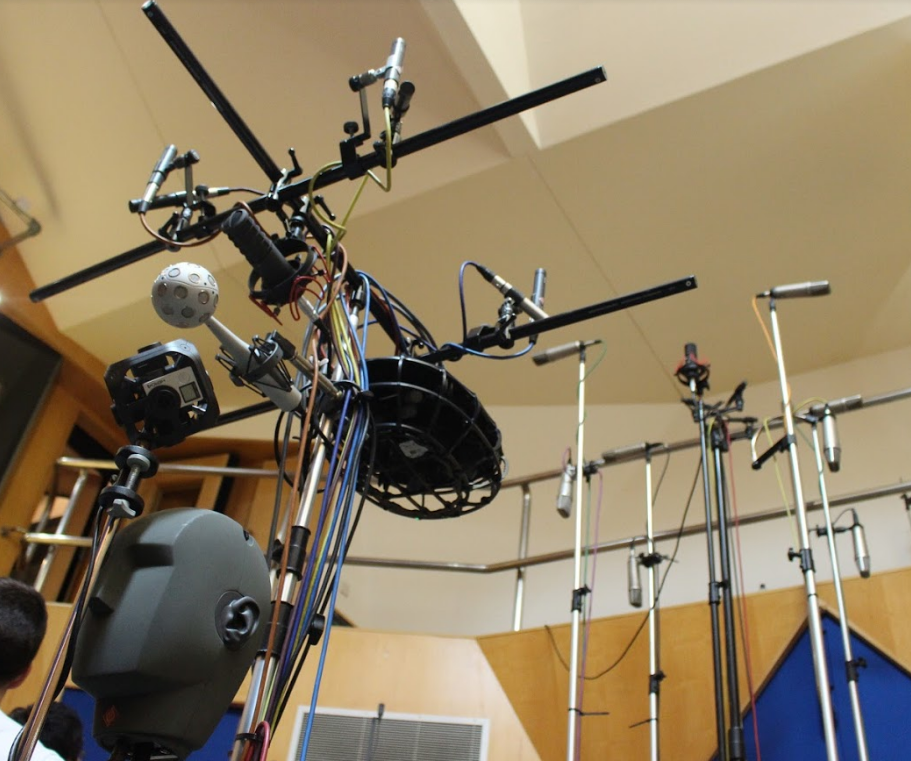
\includegraphics[width =\linewidth]{images/other/posAC.png}
				\caption{Microphones at position A with microphones in position C in the background}
				\label{AvsC}
			\end{center}
			\end{figure}

		\subsubsection{Spot Mics}

			For an ensemble such as this it is natural when performing for each musician to be spot miked due to the natural variation in dynamics. If only the microphone arrays described above were used then the lead and backing vocalists would be drowned out by the drums. As it was also decided that the bass guitar would be recorded in isolation to avoid the lower bass frequencies overpowering other sound sources within the recording space, the bass guitar would not be picked up by the arrays at all. Therefore each instrument required their own spot mic to ensure that the vocals and bass guitar could be mixed in consistently with the rest of the ensemble. The spot microphones were positioned by Abbey Road engineers using their usual recording techniques and work flow. The spot microphones and placement for each instrument are detailed below.\\
			
			\paragraph{Drums}

			Each section of the drum kit was recorded using spot microphones, the details for which are displayed in table~\ref{spots}.\\

			\begin{table}[h]
				\centering
				\resizebox{0.45\textwidth}{!}{%
				\begin{tabular}{m{15mm} lll}
					Section & Microphone Model & Polar Pattern & Position \\
					\hline
					\multirow{2}{*}{Kick Drum} & Shure Beta 52a & Cardioid & Inside the kick drum  \\
					& Neumann U47-fet & Cardioid & In front of the kick drum\\
					\hline
					\multirow{2}{*}{Snare Drum} & Shure Unidyne III 57 & Cardioid & Top of snare drum \\
					& AKG 414 & Cardioid & Underneath snare drum \\
					\hline
					Hi-Hat & Shure SM58 & Cardioid & Above Hi-Hat \\
					\hline
					Knee & Sony C38 & Cardioid & Above drummer's right knee \\
					\hline
					Mid Tom & Beyer M201 & Cardioid & Above mid tom \\
					\hline
					High Tom & Beyer M201 & Cardioid & Above mid tom \\
					\hline
					Mono Overhead & Coles 4038 & Bi-directional & Above the drummers head \\
					\hline
					Stereo Overheads & 2 x DPA 4011 & Cardioid &  Standing position for Vocalist \\
					\hline
					Stereo Drum Room Mics & 2 x DPA 4006 & Omnidirectional & 3 feet in front of the drum kit \\
					\hline
				\end{tabular}}
				\caption{A table of the spot microphones used for recording the ensemble}
				\label{spots}
			\end{table}

			\paragraph{Bass Guitar}
				To prevent excessive low frequency spill from the bass guitar, an Ampeg B15N Portaflex bass amplifier was placed in an isolation booth and recorded with a Neumann FET 57 microphone. As it would look unnatural to hear the bass but see no bass amplifier in the VR experience, a 'dummy' bass amp was placed in the room to the left of the bassist with the rest of the musicians. Figure~\ref{drums} shows the FET mic placement on the dummy amplifier. \\

				\begin{figure}[ht]
				\begin{center}
					\includegraphics[width = \linewidth]{images/other/dummycab.JPG}
					\caption{Neumann FET 57 placement on the 'dummy' amplifier}
					\label{drums}
				\end{center}
				\end{figure}

			\paragraph{Electric Guitars}
				An Orange Crush 60R amplifier and a Fender Blues Junior amplifier were placed on the right and left of the central position with both guitarists respectively. Both amplifiers were placed on chairs to raise the height and angled up to allow a clear path for sound to travel towards the multichannel microphone arrays and Ambisonic microphones. Neumann U87 condenser microphones were also placed centrally in front of the amplifiers. Direct signals were also taken from both guitarists pedal boards. Effort was made to match the volumes of both guitar amplifiers to create a balanced sound within the room which would be captured by the multichannel microphone arrays. Figure~\ref{guitarAmps} shows both of the electric guitar amplifiers as described.\\

				\begin{figure}
					\centering
					\subfloat[][Neumann U87 placement on Guitar 1 amplifier]{
						\includegraphics[width=.5\linewidth]{images/other/gtr1.JPG}
						\label{fig:sub1}}
					\subfloat[][Neumann U87 placement on Guitar 2 amplifier]{
						\includegraphics[width=.5\linewidth]{images/other/gtr2.JPG}
						\label{fig:sub2}}
					\caption{Spot microphones on the electric guitar amplifiers}
					\label{guitarAmps}
				\end{figure}
				

			\paragraph{Vocals}
				The lead vocalist was recorded using a Shure SM7B microphone and positioned to the right of the drum kit, shown in figure~\ref{voxmic}. Acoustic panels were placed between the drums and vocalist to minimise any spill picked up by the vocal microphone. Backing vocals provided by guitarist 2 were also recorded using a Shure SM7B, whilst the drummers backing vocals were recorded using a Shure SM58. Microphone directivity was crucial to reject as much off-axis sound as possible.\\

				\begin{figure}[ht]
				\begin{center}
					\includegraphics[width = \linewidth]{images/other/vox.JPG}
					\caption{Picture showing the placement of the Shure SM7 and acoustic panels}
					\label{voxmic}
				\end{center}
				\end{figure}


	\subsection{Recording Process}
		Once the equipment was set-up for the recording session, each of the microphone channels from each multichannel microphone array and Ambisonic microphone were connected to tie lines in the live room and routed to a channel on the SSLJ 9000J 96-channel mixing console in the control room. The spot microphones used the pre-amplifiers on the mixing console as did each channel of the Hamasaki Cube. For the Ambisonic microphones (Soundfield ST450 and Sennheiser AMBEO), a stepped pre-amplifier was required to ensure that the gain levels set for each of the W, X, Y and Z channels were identical. There were thirty six AMS Neve Montserrat pre-amplifier channels and twelve AMS Neve 1081 pre-amplifier channels available for the session. Care was taken to ensure that each microphone array and Ambisonic microphone used the same pre-amp model for each of their individual channels. 

		The session was recorded on a ProTools HD rig \cite{ProToolsHD} at a sampling rate of 48kHz and a bit-depth of 24. This was the practical option as there were in excess of ninety channels being used and the file sizes had to be taken into consideration. Recording at 48kHz/24bit allowed for high-quality recordings whilst ensuring that the file sizes were still practical to work with in the post-production process. The Eigenmike was recorded onto a separate laptop that was synchronised to the ProTools HD session and time-stamped, allowing for the Eigenmike to be recorded simultaneously with the ProTools HD session.

		A 5.1 surround system comprising of five Bowers and Wilkins 800D speakers was used for monitoring in the control room. Where possible, the arrays were 'folded down' to the 5.1 system for monitoring. The spot microphones were monitored in stereo as would be the case in a conventional recording session. Although the monitoring system did not allow for 3-D audio reproduction, it was useful to listen and switch between each of the different channels and different microphone arrays in real-time. Timbral qualities such as the brightness of the microphones could be identified whilst monitoring and it provided an early indication to how each of the different multichannel microphone arrays and Ambisonics microphones might sound after the implementation stage.

		%\section{Recording Summary}

		%Including the Eigenmike there were 122 channels that needed to be recorded simultaneously in the session for each performance. A session of this size required meticulous planning and attention to detail to ensure everything was set-up, documented, routed and recorded successfully. Due to the size of the session, no one person was in a position to have a clear overview of the whole recording process. For each take the cameras needed to be checked and set to record, the band needed to be given feedback and each input channel had to be monitored to ensure that everything was being recorded as planned. Only as a team was it possible to undertake such an intensive audio and visual recording session in one day.